\documentclass[conference,letterpaper]{IEEEtran}

\usepackage{fontspec}
\usepackage{hyperref}
\usepackage[style=ieee,backend=biber]{biblatex}
\addbibresource{report.bib}

\usepackage{tikz}
\usetikzlibrary{shapes,decorations,arrows,positioning,fit}
\tikzset{point/.style={circle,draw,fill=black,radius=2pt}}
\tikzset{cpoint/.style={circle,draw,fill=white,radius=2pt}}
\tikzset{>=stealth',thick}

\usepackage{fancyhdr}
\usepackage{lastpage}
\usepackage{flushend}
\usepackage{algorithm}
\usepackage{algpseudocode}
\algrenewcomment[1]{\(\triangleright\) #1}

\renewcommand{\headrulewidth}{0pt}
\cfoot{Page {\thepage} {of} {\pageref{LastPage}}}

\title{Multi-Agent Continuous Motion Simulation using Discrete Events}
\author{%
    Jack Rosenthal \\
    Colorado School of Mines \\
    Computer Science Department \\
    \texttt{jrosenth@mines.edu}
    \and
    Qin Yang \\
    Colorado School of Mines \\
    Computer Science Department \\
    \texttt{qinyang@mines.edu}}

\rhead{Rosenthal and Yang, 2018}


\hypersetup{
    pdfauthor={Jack Rosenthal and Qin Yang},
    pdftitle={Multi-Agent Continous Motion Simulation using Discrete Events},
    pdfsubject={Computer Simulation Techniques}
}

\usepackage{amsmath}
\usepackage{amssymb}
\let\le=\leqslant
\let\ge=\geqslant

\begin{document}

\maketitle
\thispagestyle{fancyplain}
\pagestyle{fancyplain}

\begin{abstract}
    Multi-agent systems with continuous motion (such as swarm robotics systems)
    are often simulated in a time-step agent-based simulation system due to the
    relative ease of implementing an emergent behavior in agent-based
    simulations. The disadvantage of this approach is that simulation accuracy
    is proportional to the size of the time-step in the system, and as the size
    of the time-step decreases, the computational time required to run the
    simulation increases.

    Our paper proposes a modified discrete event simulation technique for
    simulating many agents operating in the same continuous space. We do so by
    adding two new techniques to a discrete event simulation we call
    \emph{cross-cutting} and \emph{cancellation}. Finally, we provide an
    evaluation of the computational complexity of our modified discrete event
    simulation technique when compared to time-step agent-based simulations
    through a simple swarm robotics scenario.
\end{abstract}

\section{Introduction}

Simulating continuous motion of many agents in the same space is non-trivial to
implement, as the motions of one agent may depend on the motions of the
surrounding agents. Often times, the system may be thought of using emergent
behaviors; that is, each agent follows a simple set of rules in order to
accomplish a behavior much greater than the sum of its parts.

Emergent behaviors are easy to implement in a time-step agent-based simulation,
as the individuals behaviors can simply be encoded as a set of predicates and
the resulting transition to the agent at each time step. While this model has
the advantage of easy implementation and trivial verification, it is not very
computationally efficient as the computational time required is proportional to
the amount of steps in the simulation.

Certain multi-agent systems \emph{need} to be encoded using a time-step
agent-based simulation. For example, consider Conway's Game of
Life \cite{conway}, a cellular automaton: each agent fundamentally may only make
a plan for the next step in the simulation by the very nature of the game. But
in some systems, agents may plan for a continuous motion and only adjust their
plan when they need to. For example, a driver of a vehicle may have their
entire route planned ahead of time, but may have to make changes based on their
simple rules for driving on the road (avoid accidents with other vehicles,
don't drive on closed roads, etc.) For the latter kind of simulation, we can
save computational time and improve simulation accuracy by implementing as a
discrete event simulation rather than a time step model, at the cost of reduced
implementation ease, and significantly reduced ease of verifying the
computational model.

This paper extends the traditional discrete event simulation model by adding
two new techniques to support continuous motion simulation with multiple
agents:
\begin{enumerate}
    \item Events may now be \emph{cancelled}. In terms of a typical discrete
        event simulation software system, this means that previously scheduled
        events may be removed from the event queue (or are otherwise prevented
        from being processed) before they are processed.
    \item Events must provide \emph{cross-cutting}. In terms of a typical
        discrete event simulation software system, events which interfere with
        the completion of other events must trigger the cancellation and
        rescheduling to occur.
\end{enumerate}

Our paper implements these techniques for modeling continuous motion of
multiple agents under the following technique:
\begin{enumerate}
    \item When a simulation agent $A$ makes an initial plan, they schedule an
        event $E_{A1}$ indicating the planned time of arrival at the desired
        position and create continuous functions which will represent their
        position and distance traveled with respect to the simulation clock as
        they move to that position.
    \item When a simulation agent $B$ executes an event $E_{B1}$ which
        cross-cuts (prevents) $A$'s plan from completing as intended,
        simulation agent $A$ will devise a new plan, evaluating their
        previously derived continuous position and distance functions, updating
        their distance traveled accordingly, and derives new position and
        distance traveled functions from their previously evaluated position.
        $A$ will then schedule the new event $E_{A2}$ indicating their new plan
        for arrival.
\end{enumerate}
Figure~\ref{fig:introagentfunctions} shows a scenario derived from above
example in a picture.

\begin{figure}[ht]

    \begin{center}
    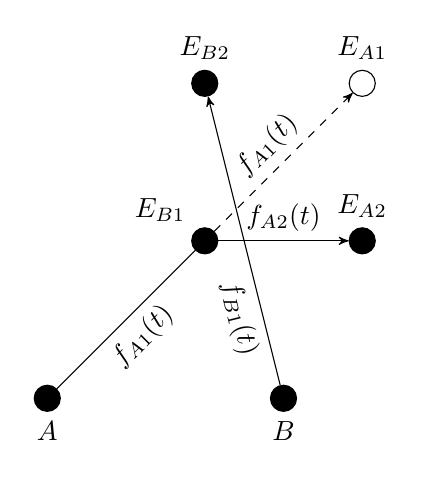
\begin{tikzpicture}
        \node[point,label=below:{$A$}] (Ainitial) at (0,0) {};
        \node[point,label=above left:{$E_{B1}$}] (collide) at (2,2) {};
        \node[cpoint,label={$E_{A1}$}] (EA1) at (4,4) {};
        \node[point,label={$E_{A2}$}] (EA2) at (4,2) {};

        \node[point,label=below:{$B$}] (Binitial) at (3,0) {};
        \node[point,label={$E_{B2}$}] (EB2) at (2,4) {};

        \draw (Ainitial) -- (collide) node[midway,sloped,below] {$f_{A1}(t)$};
        \draw[->,dashed] (collide) -- (EA1) node[midway,sloped,above] {$f_{A1}(t)$};
        \draw[->] (collide) -- (EA2) node[midway,sloped,above] {$f_{A2}(t)$};
        \draw[->] (Binitial) -- (EB2) node[near start,sloped,below] {$f_{B1}(t)$};
    \end{tikzpicture}
    \end{center}

    \caption{Initially, agent $A$ plans on arrival at the point indicated by
    $E_{A1}$ with continuous travel function $f_{A1}(t)$. Then, agent $B$
    schedules travel to the point indicated by $E_{B2}$, but realizes this will
    cause collision with $A$, and $A$ would notice this at time $t_c$. $B$ then
    schedules $E_{B1}$ for time $t_c$ to indicate to $A$ to change the plan of
    travel. When $E_{B1}$ is executed, $A$ then evaluates $f_{A1}(t_c)$ to
    determine its position, and creates a new travel function $f_{A2}(t)$
    indicating the planned travel to the point indicated by $E_{A2}$.
    Presumably, at this point $A$ may wish to schedule another event to reach
    its initial desired position.}
    \label{fig:introagentfunctions}

\end{figure}

The remainder of the paper is organized as follows: Section~\ref{sec:related}
discusses related work in the field of both simulation, multi-agent systems,
and robotics, section~\ref{sec:statement} formally defines the problem we are
trying to solve, section~\ref{sec:technique} defines a generalized simulation
technique for implementing a discrete event simulation with multiple agents in
motion through a continous space, and section~\ref{sec:evaluation} evaluates
our simlulation technique using a scenario in swarm robotics. Finally,
section~\ref{sec:conclusion} draws conclusions from our work.

\section{Related Work}
\label{sec:related}

Swarm robotics in a new and rising field, and many simulators for swarm
robotics systems have been developed. For example, ARGoS \cite{argos}, Gazebo
\cite{gazebo}, USARSim \cite{usarsim}, Webots \cite{webots}, and MuRoSimF
\cite{murosimf} are all simulators for multi-robot systems. However, all of
these simulators use a time-step agent-based model for their simulations. Our
computational model is implemented using a discrete event simulation (see
\cite[p.~3]{leemispark} for the definition of a discrete event simulation),
which is a fundamentally different simulation model than all of the previously
mentioned simulators. To our knowledge, we are the first to simulate a
multi-agent robot system using a discrete event simulation.

\emph{Cancellation} is not a new technique in discrete event simulations.
\cite{schruben1983} includes canceling edges in their event graph theory, and
even \cite{elimcancel1} and \cite{elimcancel2} both show how canceling events
can be eliminated from a simulation model: cancellation is merely a convenience
from a software standpoint. To our knowledge, we are the first to take
advantage of cancellation in discrete event simulations to make multi-agent
continuous motion possible.

\section{Problem Statement}
\label{sec:statement}

Our problem can be formally defined as followed:

\begin{quote}
    Given $N\ (N \ge 2)$ agents in a shared $k$-dimensional $(k \ge 2)$
    coordinate system, for which the agents preform some amount of planning
    that may change, devise a generalized technique used to implement a
    discrete event simulation of the agents motion in the continuous space.
\end{quote}

In addition, we will discuss technique to prevent collision of agents in the
space, although this is not always needed (for example, a colony of ants often
times will climb on top of each other, so the technique allows for simulation
of agents directly on the same point).

\section{Simulation Technique}
\label{sec:technique}

In order to discuss the techniques for writing a discrete event simulation of
multiple agents in a continuous space, we must first define the common action
of the agents: \emph{travel}. While in the real world, travelling and planning
algorithms may be implemented continuously, or in a time-step based simulation
from step-to-step, we must extend the traditional definitions of travel to
support usage in a discrete event simulation:

\begin{quote}
    \textbf{Travel:} travel is the act of \emph{planning a complete path} from
    one position (the start) to another (the goal), and attempting to execute
    that plan at least partially, completing the plan unless another reason
    arises.
\end{quote}

For an agent to preform travel, they must take advantage of our
\emph{cross-cutting} method. Our cross-cutting method is outlined in
Algorithm~\ref{alg:crosscut}.

\begin{algorithm}
    \caption{Cross-cutting Travel Algorithm}
    \label{alg:crosscut}

    \begin{algorithmic}
        \Procedure{InitializeAgent}{$A, A_i$}
            \State \Comment{The agent must have an initial cross-cutting function when
            it is created}
            \State $p_A(t) \gets t \mapsto A_i$
        \EndProcedure

        \Procedure{Travel}{$A, A_n, c, P$}
            \State \Comment{Agent $A$ plans travel to point $A_n$ at time $c$ with
            planning function $P$}
            \State \Comment{Before updating the cross-cutting function, the simulation
            may want to make note of other intermediate variables, such as
            distance traveled}
            \State $p_A(t) \gets P(p_A(c), A_n)$
            \ForAll{$B$, where $B$ is an agent and not ourselves}
                \State{Symbolically determine if $B_p(t)$ has an intersection with
                $A_p(t)$}
                \State{Schedule cancellation and notice events appropriately}
            \EndFor
        \EndProcedure
    \end{algorithmic}
\end{algorithm}

\subsection{Planning Considerations}

While Algorithm~\ref{alg:crosscut} is sufficient to prevent collision, it
always considers the agent who scheduled travel after another to have the
precedence in collision avoidance.

In order to avoid rescheduling the initial agent's travel, the planning
algorithm used may wish to consider the travel of the other agents in the
system and plan around some (or all) of their routes. Taking this into account,
the precedence of the agents in the system can be considered in any order.

\section{Evaluation: Using a Simple Swarm Robotics Scenario}
\label{sec:evaluation}

To evaluate the effectiveness of our generalized simulation approach, we
implement a simple scenario in swarm robotics to simulate using our techniques:
\begin{itemize}
    \item \textbf{Robots} are the agents in the system. Each robot has a
        continuous 2-dimensional position, and maintains an internal state of
        the distance traveled.
    \item \textbf{Tasks} appear at specified times and locations. Each task has
        a defined \textbf{radius}, which specifies the distance at which the
        task may be circled in order to preform work on it.
    \item When a task appears, a selected set of robots goes to the task to
        preform work on it. When all robots selected are at the task, they
        begin circling around it. The selection function can be any
        partitioning function, but we implement as a simple \emph{split into
        $k$ partitions based on robot id} algorithm\footnote{This approach may
        seem too simple, but we are using this to test and evaluate the
        effectiveness of our simulation technique rather than of our planning
        technique. If one were using our simulation technique to implement a
        novel planning algorithm, presumably, this approach would be better.}
\end{itemize}

We define the following event types to handle this simulation:
\begin{itemize}
    \item \texttt{RobotCreated}: A new robot has appeared in the system, and
        its initial cross-cutting function has been set.
    \item \texttt{TaskCreated}: A new task has been created. This event
        causes the robots to partition and spawns \texttt{BeginTravelToTask}
        events for the robots who travel to the task.
    \item \texttt{BeginTravelToTask}: The robot has begun travel to a task, and
        has scheduled an \texttt{ArrivalAtTask} for when it plans to arrive.
        The cross-cutting function is evaluated to determine current position,
        and the internal distance measure of the robot is updated accordingly.
        This event has the ability to cancel events, as the robot may not be
        travelling to where it was originally.
    \item \texttt{ArrivalAtTask}: The robot has arrived at the task, and is
        ready to begin work. If all robots have arrived at the task, a
        \texttt{TaskBegin} event is created. This event may be cancelled, as
        simulation agents may begin travel to another task once they are
        already on the way to the task.
    \item \texttt{TaskBegin}: All robots have arrived at the task, and work
        begins on the task. When this happens, the cross-cutting function of
        the robot has been updated to reflect their motion in a circle around
        the task. This event may be cancelled for the same reasons as
        \texttt{ArrivalAtTask}.
\end{itemize}

Figures \ref{fig:simstart}, \ref{fig:sim73}, and \ref{fig:simlast} show a
visualization of the various parts of the simulation.

\begin{figure}[ht]
    \includegraphics[width=\linewidth]{sim1.pdf}

    \caption{At the beginning of the simulation with $N = 9$ robots, the robots
    start on the left hand side.}
    \label{fig:simstart}

\end{figure}

\begin{figure}[ht]
    \includegraphics[width=\linewidth]{sim73.pdf}

    \caption{At $t = 1$, task $1$ appears, and the robots navigate to the
    task.}
    \label{fig:sim73}

\end{figure}

\begin{figure}[ht]
    \includegraphics[width=\linewidth]{sim468.pdf}

    \caption{As new tasks appear, the robots partition themselves amongst the
    tasks.}
    \label{fig:simlast}
\end{figure}

We implemented the simulation in Python 3.6 and used Python's \texttt{heapq}
module for our underlying event queue data structure. The simulation software
can be obtained at the following URL:

\url{https://github.com/jackrosenthal/swarm-des}

\subsection{Performance Evaluation}

The discrete event simulation technique will outperform a time-step based
technique (arbitrarily) when large intervals are placed between different tasks,
as the time-step simulation has to simulate the intermediate time intervals.
But how does the simulation preform when given closely-spaced tasks (resulting
in a large number of canceled events)?

To answer this question, we tested with $2$ tasks placed at the same time. This
causes the robots to initially schedule the first scheduled task, then half of
the robots will have to cancel an event and go to the second task instead.

Tests were preformed on Intel® Core™ i7-6700K CPU at $4.00$ GHz running Linux.
Results for this selected set of parameters can be seen in
Table~\ref{tbl:times}. Note that these selected set of parameters was an edge
case designed to cause many cancellations and is not representative of the
overall performance of the simulation.

\begin{table}[hb]
    \caption{Overlapping Tasks: Performance}
    \label{tbl:times}
    \begin{center}
    \begin{tabular}{| c | c |}
        \hline
        \textbf{Robots} & \textbf{Execution Time} (seconds) \\
        \hline
        $50$ & $0.06$ \\
        \hline
        $100$ & $0.09$ \\
        \hline
        $500$ & $0.36$ \\
        \hline
        $1000$ & $1.13$ \\
        \hline
        $2000$ & $4.24$ \\
        \hline
        $5000$ & $18.61$ \\
        \hline
    \end{tabular}
    \end{center}
\end{table}

The notable decay in performance is a result of the large heap event queue with
cancelled events sitting in it. Performance for this edge case could be
increased by switching to a more efficient data structure for event list
management (such as \emph{Henriksen's Algorithm} \cite{henriksen}, a hybrid
data structure overlaying a binary search tree on a linked list) or even
eliminating cancellation from the simulation model \cite{elimcancel1}.

\section{Conclusion}
\label{sec:conclusion}

Our work introduces discrete event simulation to the simulation of
continuous multi-agent systems, a field which previously only implemented
simulations using time-step based models. By doing so, implementers of
simulations are able to simulate their models for time scales which would be
infusible in a time-step simulation.

Implementing in a discrete event simulation does have a number of drawbacks:
\begin{enumerate}
    \item Developing the computational model requires significantly more
        effort: extra care must be taken to developing appropriate planning
        algorithms for the simulation rather than simply encoding the agent's
        logic for each time-step.
    \item Verification of the computational model is no longer trivial as it is
        with time-step agent-based simulations. We verified our computational
        model using a visualization to ensure that the cross-cutting functions
        behaved as we thought we had made them. Developing better verification
        procedures for computational models of these systems could be further
        work in this area.
\end{enumerate}

Simulation is important to the field of robot planning. By implementing motion
planning algorithms in simulation (especially stochastic algorithms), the
performance of the planning algorithm can be evaluated without the need for
many expensive robots. By implementing in a discrete event simulation, time
scales which would be infeasible in traditional time-step simulations become
computable, at the cost of reduced ease of implementation and verification.

\printbibliography

\end{document}
